\chapter{算法实现}
\markboth{正文}{正文}

第一章的分析指出,现有研究已经证明了单目深度估计在改善深度图像超分辨率重建性能方面的有效性,但不足的是并没有明确地探究两个任务的相关性。与之前的工作不同,本文提出了单目深度估计和深度图像超分辨率重建的联合学习网络(BridgeNet),以实现更好的深度图像超分辨率重建性能。

本文提出的联合学习网络是基于第二章所陈述的理论和技术构建的,本章将按照自顶向下的逻辑,由网络的整体到局部分层进行介绍。首先将介绍本文提出的单目深度估计和深度图像超分辨率重建的联合学习网络(BridgeNet)的网络架构及训练策略,然后将介绍用于子网络间交互的桥接器的设计动机和模块功能。

\section{网络架构}

图 \ref{fig:fig3-1} 描述了本文提出的单目深度估计和深度图像超分辨率重建联合学习网络(BridgeNet)的总体架构,该网络由两个子网络(即深度图像超分辨率重建子网络和单目深度估计子网络)和两个桥接器(即高频注意力桥和内容引导桥)组成。将深度图像超分辨率重建子网络(DSRNet)和单目深度估计子网络(MDENet)集成到一个统一的框架中,以实现深度图像超分辨率重建和单目深度估计的联合学习,并分别将高频注意力桥(HABdg)和内容引导桥(CGBdg)应用于网络的编码器和解码器,以将这两个任务桥接在一起。

\begin{figure}[!htbp]
%	\vspace{-0.8cm}  %调整图片与上文的垂直距离
	\centering
	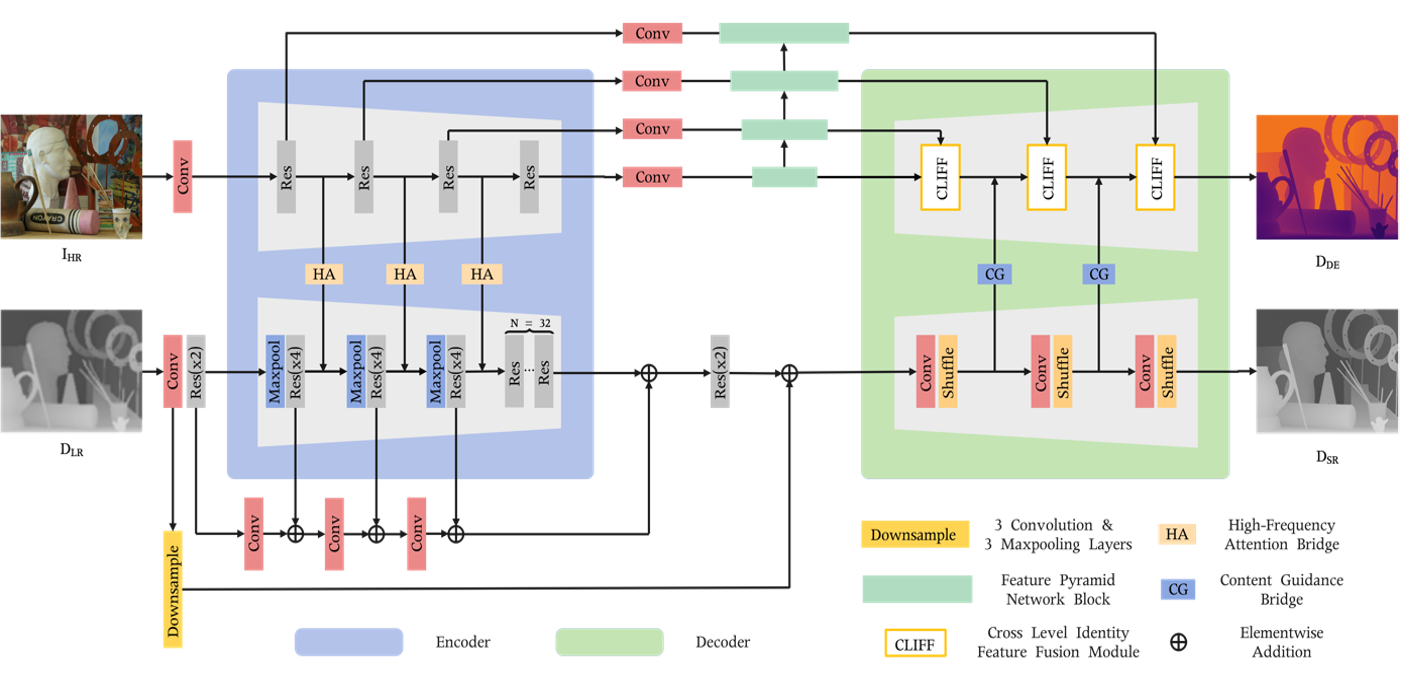
\includegraphics{figures/17.png}
	\caption{单目深度估计和深度图像超分辨率重建联合学习网络(BridgeNet)架构}
	\label{fig:fig3-1}
	\vspace{-0.8cm}  %调整图片与下文的垂直距离
\end{figure}

\newpage
给定一组高分辨率的 RGB-D 图像对 $\{I_{HR}^{\left(n\right)},D_{HR}^{\left(n\right)}\}_{n=1}^N$ 和相应的低分辨率深度图像 $\{D_{LR}^{\left(n\right)}\}_{n=1}^N$ 作为训练数据,其中 $N$ 是训练图像的数量。此外,低分辨率深度图像在输入网络前被插值到高分辨率深度图像的大小。本文提出的网络以低分辨率深度图像($D_{LR}$)和相应的高分辨率彩色图像($I_{HR}$)作为输入,同时对深度图像超分辨率重建子网络和单目深度估计子网络进行训练。超分辨的深度图像($D_{SR}$)是本文网络的主要输出,此外,估计的深度图像($D_{DE}$)也作为辅助输出。

\subsection{单目深度估计子网络}

编码器-解码器(Encoder-Decoder)结构在单目深度估计任务上取得了巨大的成功。本文遵循现有工作 \cite{DBLP:conf/eccv/WangZWLR20} 中使用的编码器-解码器网络结构作为本文联合学习网络的单目深度估计子网络,该子网络由三个部分组成,即特征提取器,特征金字塔网络和深度预测模块。

特征提取器从输入的彩色图像中提取出多种分辨率的多级特征图的集合。然后,通过横向连接将生成的特征图馈送到特征金字塔网络中。特征金字塔网络将提取的语义信息从高层特征传播到低层特征,进而生成优化后的多级特征,即特征金字塔。深度预测模块基于特征金字塔完成最终的深度估计。本文采用经过预训练的 ResNet-50 网络的前5层作为单目深度估计子网络的特征提取器。

为了充分利用特征金字塔,现有的一些方法采用直接融合的策略。在这种策略的指导下,首先将特征金字塔中的所有特征图上采样到相同的分辨率,然后级联在一起用于估计深度图像。尽管具有丰富语义信息的高层特征所估计的深度图像鲁棒性更强,但从非常低的分辨率直接对它们进行上采样,会由于上采样特征图的模糊而导致所估计的深度图像也很模糊。

另一种策略是对特征金字塔中不同分辨率的特征渐进式地融合。这种方法首先对高层特征进行逐步上采样,然后与相同分辨率的低层特征进行融合。虽然这样的融合方式可以在一定程度上抑制在深度估计时的模糊问题,但其输出特征主要受低级特征所决定,而这样的特征对于较难估计的场景并不具有鲁棒性。

在本文的单目深度估计子网络特征解码期间,跨层恒等特征融合(Cross-level Identity Feature Fusion, CLIFF)模块用于逐步融合优化的多层特征并完成深度估计,其结构如图 \ref{fig:fig3-2} 所示。跨层恒等特征融合模块以高层特征图和低层特征图作为输入。首先使用双线性插值(Bilinear Interpolation)将高层特征图进行上采样,使得输入的两个特征图具有相同的分辨率。由于高层特征具有丰富的语义信息且噪声更少,因此借用注意力机制的思想,通过将低层特征与高层特征相乘来对低层特征进行强化。如此一来,低层特征中的准确响应得到进一步的增强,而噪声响应则会受到抑制。为了得到高层特征、原始的和强化后的低层特征的最佳组合,跨层恒等特征融合模块通过两个卷积层来对三个特征进行进一步选择。

\begin{figure}[!htbp]
%	\vspace{-0.8cm}  %调整图片与上文的垂直距离
	\centering
	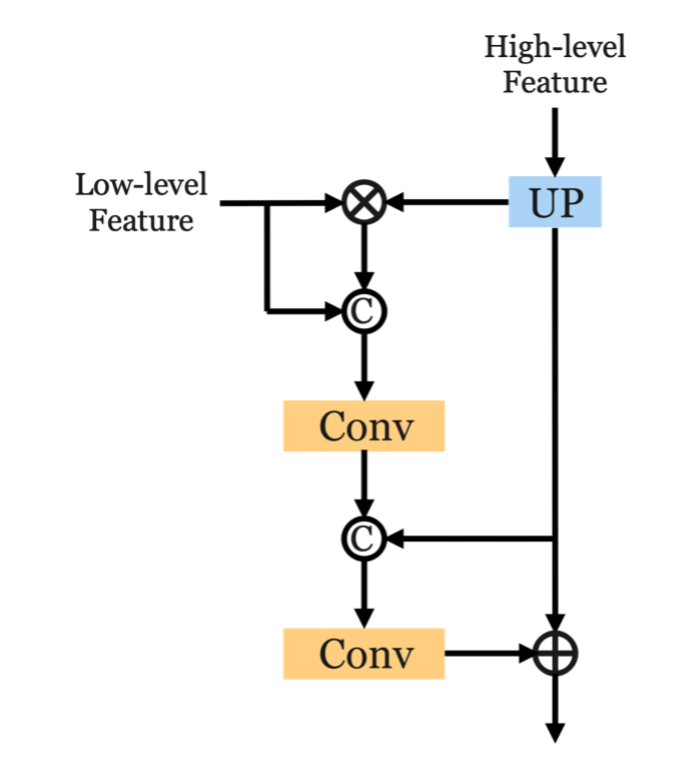
\includegraphics{figures/18.png}
	\caption{跨层恒等特征融合模块结构图}
	\label{fig:fig3-2}
	\vspace{-0.8cm}  %调整图片与下文的垂直距离
\end{figure}

具体而言,原始的低层特征和强化后的低层特征在级联后将作为第一个卷积层的输入,而第一个卷积层用于学习从级联的特征中提取更有用的信息。其输出将与高级特征级联起来,用作第二个卷积层的输入,从而实现对低层特征和高层特征的选择与聚合。此外,出于保留高级语义特征的考虑,在上采样的高层特征与第二个卷积层的输出特征之间添加了恒等映射(Identity Mapping)。通过跨层恒等特征融合模块得到的特征,兼顾了高层特征的语义信息和低层特征的结构信息,是对单目深度估计最有利的特征组合。
跨层恒等特征融合模块中所进行的操作可以描述为式 \ref{equ:equ3-1} 至式 \ref{equ:equ3-4}。

\begin{equation}
	F^a=F^l\odot F^h
	\label{equ:equ3-1}
\end{equation}
\vspace{-0.8cm}
\begin{equation}
	F_1^c=W_1\left(\left[F^l,F_a\right]\right)
	\label{equ:equ3-2}
\end{equation}
\vspace{-0.8cm}
\begin{equation}
	F_2^c=W_2\left(\left[F_1^c,F^h\right]\right)
	\label{equ:equ3-3}
\end{equation}
\vspace{-0.8cm}
\begin{equation}
	F^o=F_2^c+F^h
	\label{equ:equ3-4}
\end{equation}

\noindent 式中,$F^l$,$F^a$,$F^h$ —— 原始的和强化后的低层特征及高层特征;\newline
 \indent\quad $F_1^c$,$F_2^c$,$F^o$ —— 两个卷积层的输出及最终输出;\newline
 \indent\quad $W_1$,$W_2$ —— 两个卷积层的权重;\newline
 \indent\quad $\odot$ —— 像素级相乘;\newline
 \indent\quad $[·,·]$ —— 级联操作。
 
 \newpage
 
 \subsection{深度图像超分辨率重建子网络}
 
 遵循人脸超分辨率网络的结构 \cite{DBLP:conf/aaai/YinRZF20},本文同样将编码器-解码器网络作为深度图像超分辨率重建的基线。其中,编码器由一个浅层特征提取器(包含一个卷积层和一个残差块)和三个连续的特征编码模块以及一些堆叠的残差块构成。每个特征编码模块由一个最大池化层和四个串联的残差块组成,残差块的结构如图 \ref{fig:fig3-3} 所示。最大池化层可以确保深度图像超分辨率重建子网络编码器每一层的特征与单目深度估计子网络编码器对应层特征的分辨率相同,以便后续特征指导的顺利进行。

\begin{figure}[!htbp]
%	\vspace{-0.8cm}  %调整图片与上文的垂直距离
	\centering
	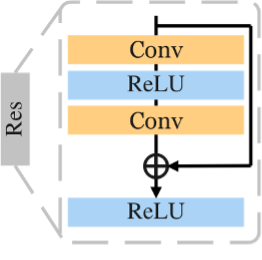
\includegraphics{figures/19.png}
	\caption{残差模块结构图}
	\label{fig:fig3-3}
	\vspace{-0.8cm}  %调整图片与下文的垂直距离
\end{figure}

在深度图像超分辨率重建子网络中,所有卷积层都使用大小相同的 $3 \times 3$ 卷积核,且每个卷积操作后面紧随一个 ReLU 激活函数。除最后的卷积层通道数设置为 3 外,子网络中其余的所有卷积操作的通道数均设置为256。深度图像超分辨率重建子网络所采用的残差模块与原始残差网络的结构基本一致,不同的是移除了残差块中的批量归一化层。

这样做的动机是由于批量归一化层(正则化层)对特征进行了归一化处理,从而导致网络丢弃了范围灵活性,所以最好是移除这些批量归一化层。现有研究 \cite{DBLP:conf/cvpr/LimSKNL17} 的实验也表明用于图像超分辨率重建的残差网络在去除所有的批量归一化层后表现最佳。不仅如此,批量归一化层会减慢网络收敛的速度,同时降低其整体性能,尤其是在图像的超分辨率重建任务中。因此在深度图像超分辨率重建子网络中,所有残差模块中的批量归一化层都被移除。

更深层的网络已经在包括图像超分辨率重建在内的许多计算机视觉任务中显示出更好的性能。增加网络的深度也是现有许多工作中使用的一种策略。经过三个特征编码模块提取出的特征将传递到由 $N$ 个残差块组成的更深层的特征提取模块中。较深的网络可以帮助超分辨的深度图像恢复出更分明的边缘和形状。
\newpage
为了恢复深度图像中的精细结构和微小物体,本文引入了多尺度策略,通过进一步融合深度图像超分辨率重建子网络编码器中间层的特征来优化高层特征。考虑到相邻层特征的相似性,并非编码器的所有特征都需要参与多尺度特征融合以形成新的特征表示,而是仅仅采用了每个特征编码模块提取的特征进行融合。因此每个最大池化层之前的特征编码模块的输出都需要通过跳连接,与深层特征模块输出的特征融合以形成具有更丰富信息的特征。此外,由于特征图每经过一个最大池化层都进行了2倍的下采样,为了匹配不同层特征图的大小,将步长为2的3×3卷积层应用于由跳连接提供的中间层特征,以实现下采样并进行特征融合。

对于低分辨率的深度图像 $D_{LR}$,上述操作可以被描述为式 \ref{equ:equ3-5} 至式 \ref{equ:equ3-7}。

\vspace{-0.4cm}
\begin{equation}
	F_0=f_0\left(D_{LR}\right)
	\label{equ:equ3-5}
\end{equation}
\vspace{-0.8cm}
\begin{equation}
	F_i=f_i\left(F_{i-1}\right),i\in\{1,2,3\}
	\label{equ:equ3-6}
\end{equation}

\noindent 式中,$F_0$ —— 通过一个卷积层和一个残差块提取的浅层特征;\newline
\indent\quad $F_i$,$i\in\{1,2,3\}$ —— 特征编码模块的输出;\newline
\indent\quad $f_0$ —— 浅层特征提取模块;\newline
\indent\quad $f_i$,$i\in\{1,2,3\}$ —— 特征编码模块。

\vspace{-0.4cm}
\begin{equation}
	F_{fusion}=g_3\left(g_2\left(g_1\left(F_1\right)+F_0\right)+F_2\right)+F_3
	\label{equ:equ3-7}
\end{equation}

\noindent 式中,$F_{fusion}$ —— 多尺度特征融合的输出;\newline
\indent\quad $g_i$,$i\in\{1,2,3\}$ —— 实现对中间层特征下采样的卷积层。

在特征解码期间,本文使用了三个顺序连接的相同上采样模块,包括一个卷积层和一个像素重组层(PixelShuffle)。特征图每经过一个上采样模块后,分辨率都变为之前的两倍。最后应用一个 $1 \times 1$ 的卷积层来重建高分辨率的深度图像。

受彩色图像超分辨率重建算法稠密残差网络(Residual Dense Network, RDN)\cite{DBLP:conf/cvpr/ZhangTKZ018} 的启发,编码器初始阶段提取的浅层特征和输入解码器的特征在进行第一次上采样前通过一个大的跳连接进行融合。设计这个跳连接的目的是为了直接提供深度图像超分辨率重建需要的低频信息,从而迫使网络更加专注于学习重建需要的高频信息而不是已经提供的低频信息。

根据网络的设计可以看到,网络提取的浅层特征图大小与上采样后的低分辨率特征图大小相同。而网络中有3个最大池化层,每个最大池化层对特征图进行因子为 $\times 2$ 的下采样,即特征图在经过编码器中三个最大池化后,分辨率下降为输入图像的1/8。为了保证长跳连接两侧的特征图拥有相同的分辨率,浅层特征被馈送到下采样(Downsample)块中以生成低频特征,然后通过长跳连接与编码器提取的最终特征相融合,下采样块的结构如图 \ref{fig:fig3-4} 所示。

\begin{figure}[!htbp]
%	\vspace{-0.8cm}  %调整图片与上文的垂直距离
	\centering
	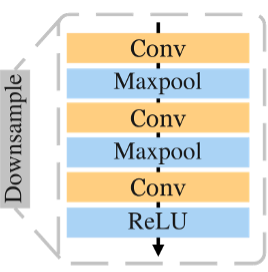
\includegraphics{figures/20.png}
	\caption{下采样模块结构图}
	\label{fig:fig3-4}
	\vspace{-0.8cm}  %调整图片与下文的垂直距离
\end{figure}

\subsection{联合学习策略}
深度图像超分辨率重建和单目深度估计具有天然的相关性,可以在同一数据集的监督下对他们进行训练。因此,这两个任务的联合学习首先体现在损失函数的联合优化上。

与其他多任务学习的损失函数为所有分支损失函数的加权和不同,本文分别为深度图像超分辨率重建和单目深度估计的损失函数分配了不同的优化器。这是因为深度图像超分辨率重建和单目深度估计的学习难度大不相同,导致两个任务的收敛速度不同,从而很难找到合适的权重设置来确保两个任务都达到最佳性能。因此,在损失函数的设计方面,本文提出分别对深度图像超分辨率重建和单目深度估计相关部分进行优化的策略。其损失函数定义为式 \ref{equ:equ3-8} 和式 \ref{equ:equ3-9}。
\vspace{-0.3cm}
\begin{equation}
	\mathcal{L}_{DSR}=||D_{SR}-D_{HR}||_1
	\label{equ:equ3-8}
\end{equation}
\vspace{-0.8cm}
\begin{equation}
	\mathcal{L}_{MDE}=||D_{DE}-D_{HR}||_1
	\label{equ:equ3-9}
\end{equation}

\noindent 式中,$\mathcal{L}_{DSR}$ —— 深度图像超分辨率重建任务的逐像素 $L_1$ 损失;\newline
\indent\quad $\mathcal{L}_{MDE}$ —— 单目深度估计任务的逐像素 $L_1$ 损失。

除了在损失函数层级对两个任务进行约束外,本文还精心设计了两个桥接器,分别将两个任务在编码器和解码器阶段相关联,以实现互利共赢。一个是编码器中的高频注意力桥(HABdg),另一个是解码器中的内容引导桥(CGBdg)。其中,高频注意力桥利用单目深度估计子网络出色的彩色特征学习能力为深度图像超分辨率重建提供指导。考虑到两个任务难度的差异,深度图像超分辨率重建子网络在解码器阶段经由内容引导桥可以为深度估计提供有效的内容指导,从而提高深度估计的性能。在以下各小节中,本文将详细介绍这两个桥接器的设计原理和实现细节。
下面给出深度图像超分辨率重建和单目深度估计联合学习网络训练策略的伪代码。

%\begin{algorithm}[H]
%        \caption{Joint Learning Strategy}
%        \LinesNumbered
%        \KwIn{Training data $D_{LR}$, $I_{HR}$, $D_{HR}$}
%        \KwOut{$D_{SR}$, $D_{DE}$}
%        Randomly initialize DSRNet and MDENet\\
%       
%        \For{ epoch=1; epoch $\leq$ 400;}
%        {
%         ——————————————— Step 1 ———————————————\\
%        $F_{MDE}=Encoder_{MDE}(I_{HR}^n)$\\
%        $F_{DSR}^{shallow}=Res^{(2)}(conv(D_{LR}))$ \tcp*{shallow feature extraction}
%        \For(\tcp*[f]{ i refers to $i^{th}$ layer of encoder}){i=1; i $\leq$ 3} 
%        {
%        \If{i=1}
%        {
%        $Fe_{DSR}^i=maxpool(Res^{(4)}(F_{DSR}^{shallow}))$\\
%        }
%        \Else{
%        $Fe_{DSR}^i=maxpool(Res^{(4)}(F_{ha}^{i-1}))$\\
%        }
%        $F_{blurred}^i=deconv(avgpool(F_{MDE}^i)$\\
%        $A_{hf}^i=PRelu(F_{MDE}^i-F_{blurred}^i)$\\
%        $F_{hg}^i=F_{MDE}^i+A_{hf}^i\cdot F_{MDE}^i$\\
%        $F_{comp}^i=[Fe_{DSR}^i,F_{hg}^i]$\\
%        $F_{ha}^i=SA(conv_{1\times 1}(CA(F_{comp}^i)))$\\
%        }
%        $F_{DSR}^{deeper}=Res^{(32)}(F_{ha}^3)$\\
%        $F_{DSR}^{multi-scale}=conv(conv(conv(Fe_{DSR}^{shallow}+Fe_{DSR}^1)+F_{DSR}^2)+Fe_{DSR}^3)$\tcp*{multi-scale features fusion}
%        $F_{DSR}^{fusion}=Res^{(2)}(F_{DSR}^{deeper}+F_{DSR}^{multi-scale})$\\
%        $F_{DSR}^{low-freq}=Downsample(F_{DSR}^{shallow})$\\
%        \For(\tcp*[f]{ j refers to $j^{th}$ layer of decoder}){i=1; i $\leq$ 3} 
%        {
%        \If{i=1}
%        {
%        $Fd_{DSR}^j=pixelshuffle(conv(F_{DSR}^{fusion}+F_{DSR}^{low-freq}))$\\
%        }
%        \Else{
%        $Fd_{DSR}^j=pixelshuffle(conv(F_{DSR}^{j-1}))$\\
%        }
%        }
%        $D_{SR}=conv_{1 \times 1}(Fd_{DSR}^3)$\\
%        Update weights of parts related to DSR with $\mathcal{L}_{DSR}=||D_{SR}-D_{HR}||_1$\\
%        ——————————————— Step 2 ———————————————\\
%        $F_{MDE}=Encoder_{MDE}(I_{HR}^n)$\\
%        \For{k=1;k $\leq$ 4}
%        {
%        \If{k=1}
%        {
%        $Fp_{MDE}^k=conv(Fe_{MDE}^{5-k})$
%        }
%        \Else
%        {
%        $Fe_{MDE}^{5-k}=interpolate(Fe_{MDE}^{5-k})$\\
%        $Fp_{MDE}^k= conv(Fe_{MDE}^{5-k} +Fe_{MDE}^{5-(k+1)})$
%        }
%        }
%         
%        \For{j=1;k $\leq$ 3}
%        {
%        \If{j=1}
%        {
%        $Fd_{MDE}^j=CLIFF(Fp_{MDE}^1,Fp_{MDE}^2)$\\
%        }
%        \Else
%        {
%        $M_{DSR}^j=conv_{1\times1}(Fd_{DSR}^j)$\\
%        $M_{MDE}^j=conv_{1\times1}(Fd_{MDE}^j)$\\
%        $W_{diff}^j=softmax(conv_{1\times1}(M_{DSR}^j-M_{MDE}^j))$\\
%        $F_{ca}^j=Fd_{DSR}^j+W_{diff}^j\ast Fd_{DSR}^j$\\
%        $F_{con}^j=[Fd_{MDE}^j,F_{ca}^j]$\\
%        $F_{cg}^j=SA(conv_{1\times1}(CA(F_{con}^j)))$\\
%        $Fd_{MDE}^j=CLIFF(F_{cg}^j,Fp_{MDE}^{j+1})$\\
%        }
%        }
%        $D_{DE}=interpolate(conv_{1\times 1}(Fd_{MDE}^3))$\\
%        Update weights of parts related to MDE with $\mathcal{L}_{MDE}=||D_{DE}-D_{HR}||_1$
%        }
%\end{algorithm}

\begin{figure}[!htbp]
	\centering
	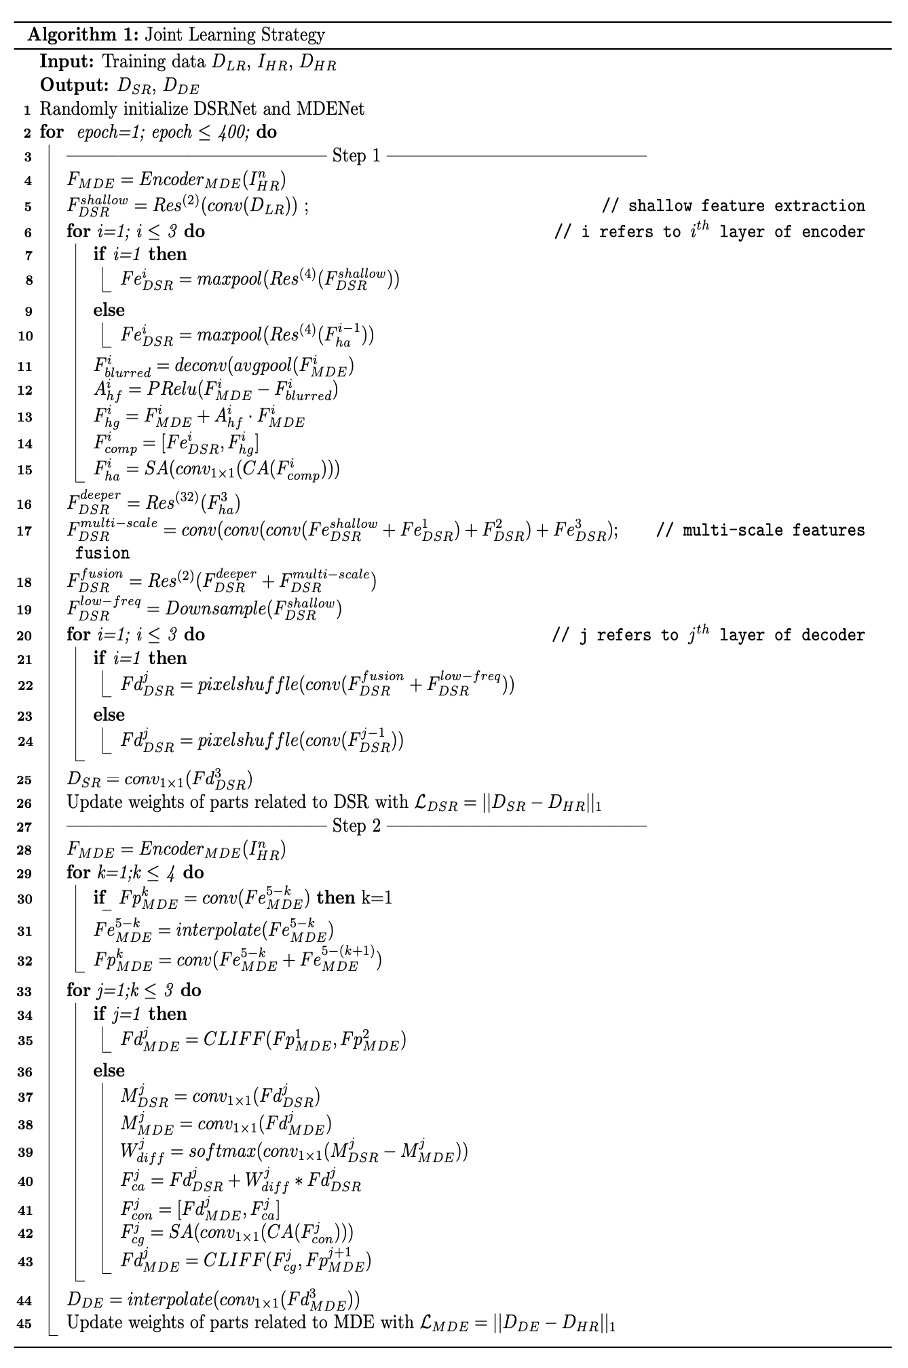
\includegraphics{figures/21.png}
\end{figure}

\section{高频注意力桥}

回顾现有的颜色指导的深度图像超分辨率重建的方法可以发现,彩色图像的指导主要包括对应特征的直接引导 \cite{HuiLT16, LutioDWS19, DBLP:journals/tip/GuoLGCFH19} 或边缘细节的引导 \cite{DBLP:journals/tmm/WangXCZSY20, DBLP:conf/icassp/YeDL18}。尽管彩色图像和深度图像具有很强的结构相似性,但是彩色图像丰富的纹理和边缘并不总是与深度图像一致,因此直接的特征引导或边缘引导可能会导致纹理复制和深度流失等问题。

在联合学习视角下,单目深度估计为解决上述问题提供了新的思路。单目深度估计任务是以彩色图像作为输入,然后实现将场景从光度表示映射到几何表示,从而生成深度图像。因此,由单目深度估计编码器提供的彩色图像的特征更接近于深度模态的特征表示。由单目深度估计编码器为深度图像超分辨率重建任务提供高频信息指导时,可以避免明显的伪影。这就是本文提出在编码器阶段使用单目深度估计代替现有方法的颜色分支来指导深度图像超分辨率重建的原因。

在明确了指导信息的传递方向之后,接下来需要思考的问题便是如何有效地实现。最简单直观的方法是通过级联或相加将单目深度估计子网络相应层的特征直接传递到深度图像超分辨率重建子网络中,但这显然不是明智的方法。在单目深度估计子网络的编码器中,随着网络的深入,特征图的分辨率逐渐降低,其中高层特征具有丰富的语义信息,而低层特征则具有更多的结构信息。由于低分辨率深度图像包含的高频信息较少,因此高分辨率的彩色图像可以为深度图像超分辨率重建提供更为重要的高频信息(例如边缘细节),而不是图像的语义信息。因此,本文设计了一个高频注意力桥,该桥接器用于从单目深度估计子网络学习高频信息以用于指导深度图像超分辨率重建子网络。高频注意力桥的结构如图 \ref{fig:fig3-5} 所示。

\begin{figure}[!htbp]
%	\vspace{-0.8cm}  %调整图片与上文的垂直距离
	\centering
	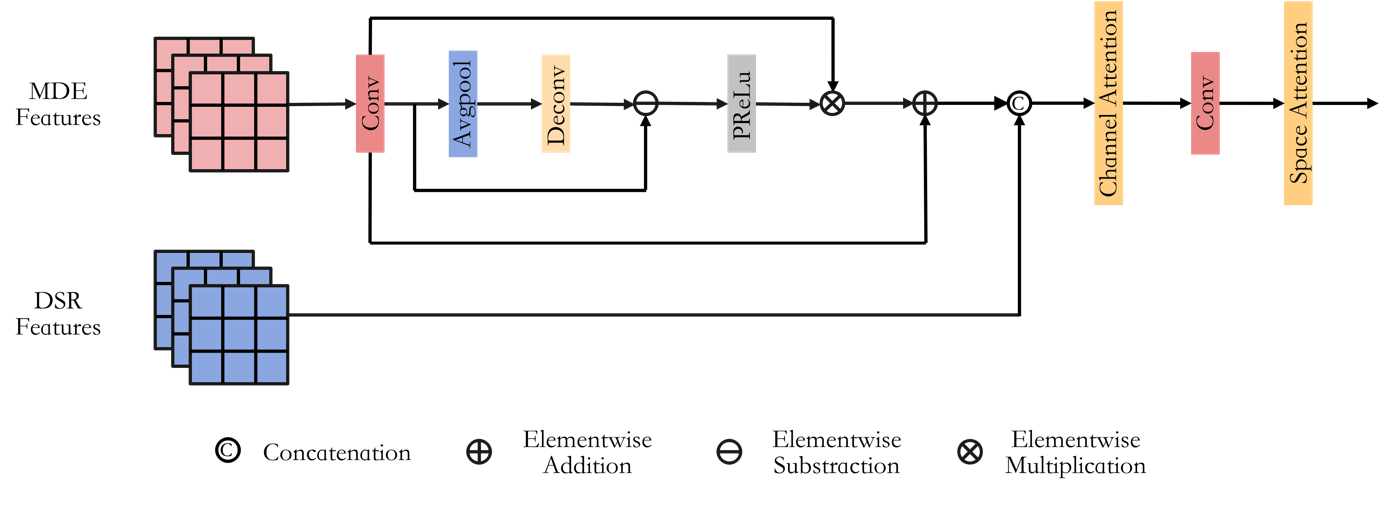
\includegraphics{figures/22.png}
	\caption{高频注意力桥结构图}
	\label{fig:fig3-5}
	\vspace{-0.8cm}  %调整图片与下文的垂直距离
\end{figure}

具体来说,首先使用平均池化和反卷积运算对单目深度估计子网络的原特征进行模糊操作,这一操作可以被描述为式 \ref{equ:equ3-10}。

\begin{equation}
	F_{blurred}^i=deconv\left(avgpool\left(F_{MDE}^i\right)\right)
	\label{equ:equ3-10}
\end{equation}

\noindent 式中,$F_{blurred}^i$ —— 获得的单目深度估计子网络第 $i$ 层的模糊特征;\newline
\indent\quad  $F_{MDE}^i$ —— 单目深度估计子网络第 $i$ 层的特征;\newline
\indent\quad $avgpool\left(\cdot\right)$ —— 平均池化操作;\newline
\indent\quad $deconv\left(\cdot\right)$ —— 反卷积操作。

然后,通过将原始特征与模糊特征相减来获得特征中的高频信息,进而生成高频信息的注意力,即式 \ref{equ:equ3-11}。

\begin{equation}
	A_{hf}^i=PRelu\left(F_{MDE}^i-F_{blurred}^i\right)
	\label{equ:equ3-11}
\end{equation}

\noindent 式中,$A_{hf}^i$ —— 获得的第 $i$ 层的高频注意力;\newline
\indent\quad $PRelu\left(\cdot\right)$ —— 带参数的修正线性单元,即激活函数。

接着,使用获得的高频注意力来对单目深度估计子网络提取的原始特征进行修正和优化,通过残差连接最终得到优化后的引导特征,即式 \ref{equ:equ3-12}。

\begin{equation}
	F_{hg}^i=F_{MDE}^i+A_{hf}^i\cdot F_{MDE}^i
	\label{equ:equ3-12}
\end{equation}

\noindent 式中,$F_{hg}^i$ —— 第 $i$ 层优化后的引导特征。

定义上述操作的原因是要在单目深度估计的原始特征中突显高频信息,以便低分辨率深度图像可以在特征融合时最大化地利用其中的高频信息。

为了利用来自单目深度估计子网络编码器优化后的指导特征,首先将它们与深度图像超分辨率重建子网络编码器相应层的特征在通道维度级联起来,以生成复合特征 $F_{comp}^i$。这种简单的特征融合在空间维度和通道维度上会有很多冗余,因此本文引入了一个注意力块,其中包括一个通道注意力 \cite{DBLP:conf/eccv/WooPLK18} 和一个空间注意力 \cite{DBLP:conf/eccv/WooPLK18} 来增强特征融合能力。通道注意力会学习每个特征通道的重要性,而空间注意会突出显示特征图中的重要位置。上述过程可以表述为式 \ref{equ:equ3-13} 和式 \ref{equ:equ3-14}。

\begin{equation}
	F_{comp}^i=\left[F_{DSR}^i,F_{hg}^i\right]
	\label{equ:equ3-13}
\end{equation}
\vspace{-0.8cm}
\begin{equation}
	F_{ha}^i=SA\left(conv_{1\times1}\left(CA\left(F_{comp}^i\right)\right)\right)
	\label{equ:equ3-14}
\end{equation}

\noindent 式中,$F_{ha}^i$ —— 深度图像超分辨率重建子网络第 $i$ 层融合高频信息的特征;\newline
\indent\quad $F_{DSR}^i$ —— 深度图像超分辨率重建子网络第 $i$ 层的特征;\newline
\indent\quad $CA$ —— 通道注意力;\newline
\indent\quad $SA$ —— 空间注意力;\newline
\indent\quad $conv_{1\times1}$ —— 卷积核大小为 $1\times 1$ 的卷积层;\newline
\indent\quad $\left[\cdot,\cdot\right]$ —— 通道维度的级联。

融合了高频信息的特征 $F_{ha}^i$ 将作为深度图像超分辨率重建子网络编码器下一层的输入。

本文采用的通道注意力模块,主要借鉴了卷积注意力机制模块(CBAM: Convolutional Block Attention Module) \cite{DBLP:conf/eccv/WooPLK18} 中通道注意力模块的设计,如图 \ref{fig:fig3-6} 所示。

\begin{figure}[!htbp]
%	\vspace{-0.8cm}  %调整图片与上文的垂直距离
	\centering
	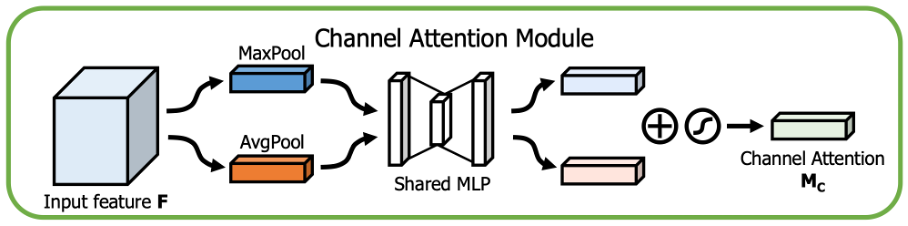
\includegraphics{figures/23.png}
	\caption{通道注意力模块结构图}
	\label{fig:fig3-6}
	\vspace{-0.8cm}  %调整图片与下文的垂直距离
\end{figure}

对于多通道特征图而言,其每一个通道都可以看作是一个独立的“特征”,因此通道注意力关注的是“对于图像而言什么特征是重要的”。为了降低学习通道注意力时的计算开销,最常用的方法是对特征图的空间维度进行“压缩”,现有的大多数工作通常只采用平均池化来聚合特征图的空间信息(如压缩-激励网络)。除平均池化外,最大池化也可用于聚合特征图所蕴含的空间信息,不同的是在梯度下降时平均池化对特征图上每一个像素点都有反馈,而最大池化只对特征图中响应最大的位置有反馈。实验表明最大池化可以挖掘到图像特征的其他重要“线索”,因而可以与平均池化合作学习得到更加有效的通道注意力。因此,本文同时使用平均池化和最大池化来对特征图的空间信息进行压缩,生成两个不同的上下文描述 $F_{avg}^c$ 和 $F_{max}^c$,然后将他们输入到一个共享的网络,并对网络的输出逐像素求和,最后经过 Sigmoid 激活函数以生成通道注意力。整个过程可以描述为式 \ref{equ:equ3-15}。

\begin{equation}
\begin{aligned}
	A^C\left(F\right)&=\sigma\left(MLP\left(AvgPool\left(F\right)\right)+MLP\left(MaxPool\left(F\right)\right)\right)\\
	&=\sigma\left(W_1\left(W_0\left(F_{avg}^c\right)\right)+W_1\left(W_0\left(F_{max}^c\right)\right)\right)
\end{aligned}
\label{equ:equ3-15}
\end{equation}

\noindent 式中,$A^C\left(F\right)$ —— 通道注意力;\newline
\indent\quad $\sigma$ —— Sigmoid 激活函数;\newline
\indent\quad $MLP$ —— 共享的网络;\newline
\indent\quad $AvgPool$ —— 平均池化操作;\newline
\indent\quad $MaxPool$ —— 最大池化操作;\newline
\indent\quad $F$ —— 特征图;\newline
\indent\quad $W_0$,$W_1$ —— 共享网络的权重。

本文采用的空间注意力模块,主要借鉴了卷积注意力机制模块(CBAM: Convolutional Block Attention Module)\cite{DBLP:conf/eccv/WooPLK18} 中空间注意力模块的设计,如图 \ref{fig:fig3-7} 所示。空间注意力是基于像素之间的空间关系产生的。与通道注意力不同,空间注意力关注的是“对于图像而言哪些位置是重要的”。类似地,本文采用平均池化和最大池化来对特征图的通道维度进行压缩,从而生成两个通道数为 1 的特征图 $F_{avg}^s$ 和 $F_{max}^s$,分别代表原始特征所有通道的平均响应和最大响应。然后将它们级联起来并通过卷积核大小为 $7\ \times 7$ 的卷积层,最后经过 Sigmoid 激活函数以生成空间注意力。

\begin{figure}[!htbp]
%	\vspace{-0.8cm}  %调整图片与上文的垂直距离
	\centering
	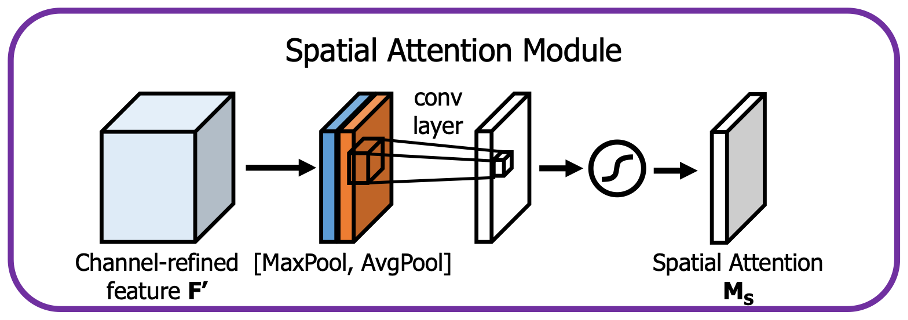
\includegraphics{figures/24.png}
	\caption{空间注意力模块结构图}
	\label{fig:fig3-7}
	\vspace{-0.8cm}  %调整图片与下文的垂直距离
\end{figure}

整个过程可以描述为式 \ref{equ:equ3-16}。

\begin{equation}
\begin{aligned}
	A^S\left(F\right)&=\sigma\left(f^{7\times7}\left([AvgPool\left(F\right);\ MaxPool\left(F\right)\right)\right)\\
	&=\sigma(f^{7\times 7}([F_{avg}^s; F_{max}^s])
\end{aligned}
\label{equ:equ3-16}
\end{equation}

\noindent 式中,$A^S\left(F\right)$ —— 空间注意力;\newline
\indent\quad $\sigma$ —— Sigmoid 激活函数;\newline
\indent\quad $f^{7\times7}$ —— 卷积核大小为 $7 \times 7$ 的卷积层;\newline
\indent\quad $AvgPool$ —— 平均池化操作;\newline
\indent\quad $MaxPool$ —— 最大池化操作;\newline
\indent\quad $F$ —— 特征图。

\section{内容引导桥}

在特征解码阶段,深度图像超分辨率重建子网络和单目深度估计子网络解码器的作用是进一步提取面向任务的特征,以完成深度估计和深度图像的超分辨率重建,最终可以从两个子网络获得相应的估计或超分辨重建的深度图像。两个任务相较而言,单目深度估计由于尺度模糊性 \cite{DBLP:conf/nips/EigenPF14} 而被广泛认知为不适定的逆问题。例如,世界上观察到的许多三维场景可以对应于完全相同的二维平面,即三维场景与二维平面之间是多对一的关系,如图 \ref{fig:fig3-8} 所示。在人眼或相机的成像过程中,大而远的物体和小而近的物体在同一成像平面上的二维信息是一致的,其前提是大物体和小物体具有相同的外观。一个很极端的例子便是现实的房间和其缩小后的展示模型。也就是说在丢失了深度信息后,想要从二维图像推理出场景的真实深度是有很大难度的,这便是尺度模糊性。

\begin{figure}[!htbp]
%	\vspace{-0.8cm}  %调整图片与上文的垂直距离
	\centering
	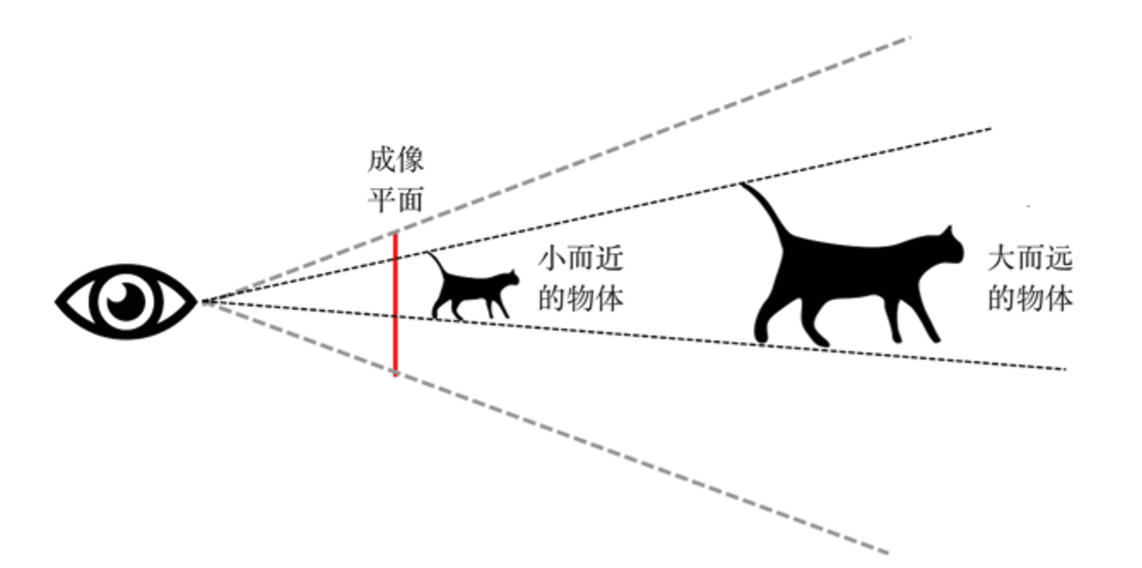
\includegraphics{figures/25.png}
	\caption{尺度模糊性示例图}
	\label{fig:fig3-8}
	\vspace{-0.8cm}  %调整图片与下文的垂直距离
\end{figure}

因此,训练一个可以很好地从彩色图像映射到深度图像的模型是一项非常艰巨的任务。尽管深度图像超分辨率重建也是一个不适定的问题,但它仍在相同的域中学习映射关系并专注于还原图像的细节,故其相对单目深度估计而言更简单。因此,由于两个任务的性能之间存在较大差距,单目深度估计子网络的解码器生成的特征不再适合为深度图像超分辨率重建的解码器提供指导信息。遵循简单任务指导困难任务的原则,本文在解码阶段交换了两个子网络的指导身份,即让深度图像超分辨率重建子网络在深度特征空间为单目深度估计子网络提供内容引导。详细结构如图 \ref{fig:fig3-9} 所示。

\begin{figure}[!htbp]
%	\vspace{-0.8cm}  %调整图片与上文的垂直距离
	\centering
	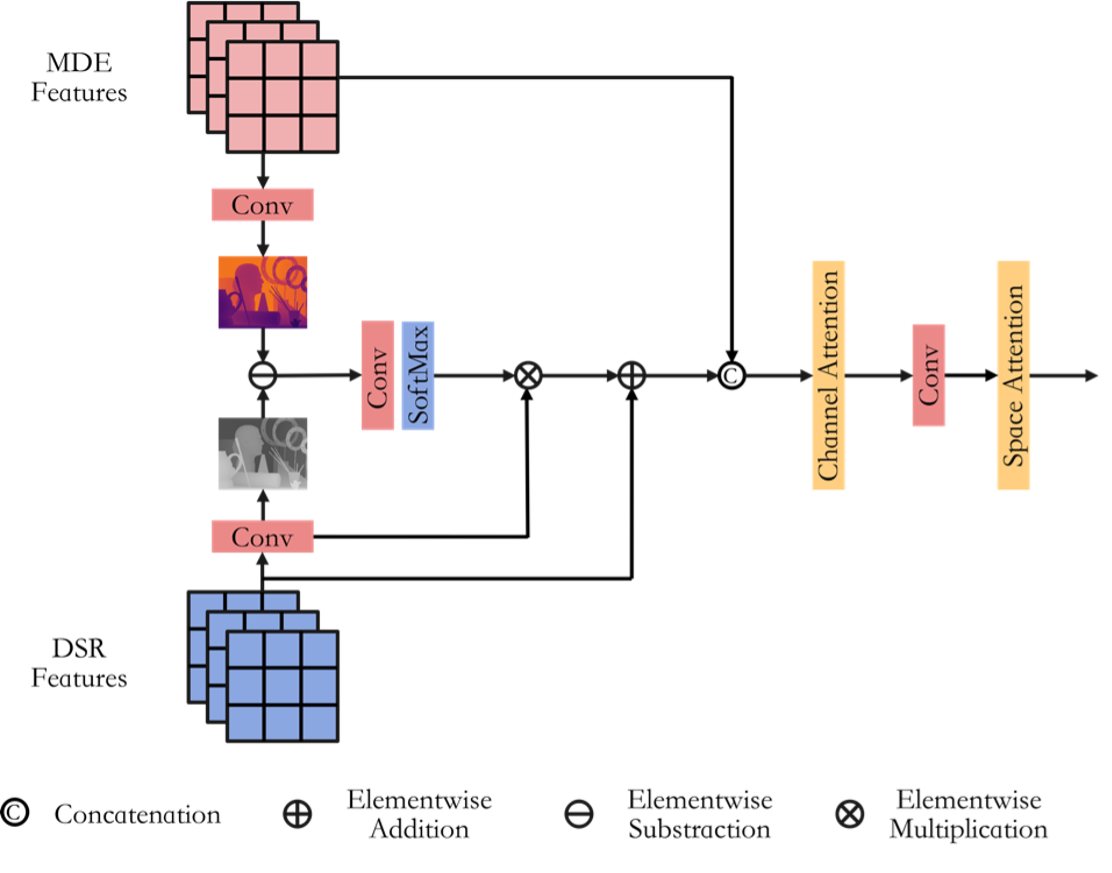
\includegraphics{figures/26.png}
	\caption{内容引导桥结构图}
	\label{fig:fig3-9}
	\vspace{-0.8cm}  %调整图片与下文的垂直距离
\end{figure}

\newpage

如前所述,本文提出的模型可以通过两个子网络的解码器特征获得相应的深度图像。具体来说,本文采用卷积核大小为 $1\times 1$ 的卷积层分别作用于深度图像超分辨率重建子网络和深度估计子网络的解码器,从而获得超分辨率的深度图像和估计的深度图像,即式 \ref{equ:equ3-17} 和式 \ref{equ:equ3-18}。

\vspace{-0.6cm}
\begin{equation}
	M_{DSR}^i=conv_{1\times1}\left(Fd_{DSR}^i\right)
		\label{equ:equ3-17}
\end{equation}
\vspace{-0.8cm}
\begin{equation}
	M_{MDE}^i=conv_{1\times1}\left(Fd_{MDE}^i\right)
	\label{equ:equ3-18}
\end{equation}

\noindent 式中,$M_{DSR}^i$ —— 深度图像超分辨率重建子网络第 $i$ 层生成的深度图像;\newline
\indent\quad $M_{MDE}^i$ —— 单目深度估计子网络第 $i$ 层估计的深度图像;\newline
\indent\quad $Fd_{DSR}^i$ —— 深度图像超分辨率重建子网络解码器第 $i$ 层的特征;\newline
\indent\quad $Fd_{MDE}^i$ —— 单目深度估计子网络解码器第 $i$ 层的特征。

然后,可以计算得到估计的深度图像 $M_{MDE}^i$ 与超分辨率重建的深度图像 $M_{DSR}^i$ 之间的差异图。差异图突出显示了估计的深度图像中相对于超分辨重建的深度图像需要进一步优化的位置,并希望这种差异会随着网络的训练越来越小。在此基础上,本文通过对差异图应用卷积运算和 softmax 激活来学习差异权重,从而为单目深度估计子网络提供内容引导。上述操作可以被描述为式 \ref{equ:equ3-19} 和式 \ref{equ:equ3-20}。

\vspace{-0.4cm}
\begin{equation}
	W_{diff}^i=softmax\left(conv_{1\times1}\left(M_{DSR}^i-M_{MDE}^i\right)\right)
		\label{equ:equ3-19}
\end{equation}
\vspace{-0.8cm}
\begin{equation}
	F_{cg}^i=Fd_{DSR}^i+W_{diff}^i\ast Fd_{DSR}^i
	\label{equ:equ3-20}
\end{equation}

\noindent 式中,$W_{diff}^i$ —— 差异权重;\newline
\indent\quad $F_{cg}^i$ —— 第 $i$ 层的内容引导特征;\newline
\indent\quad $softmax$ —— softmax 激活函数。

最后,本文使用与高频注意力桥中相同的注意力块(包含一个通道注意力和空间注意力)来优化级联的特征(即,$F_{con}^i=\left[Fd_{MDE}^i,F_{cg}^i\right]$),优化后的特征将作为单目深度估计子网络解码器中下一层 CLIFF 模块的高层特征输入,并与来自特征金字塔网络的底层特征进一步融合。

\section{本章小结}

本章从模型的组成和联合学习策略的选择,到深度图像超分辨率重建和单目深度估计两个任务间交互模式的设计进行了详细的介绍。本章介绍了深度图像超分辨率重建和单目深度估计的联合学习网络,以实现更好的深度图像超分辨率重建的性能。与现有工作[22]不同的是,在设计两个子网络之间的交互时,本文采用了更为明确的指导模式。在特征编码器中,单目深度估计子网络通过高频注意力桥为深度图像超分辨率重建子网络提供高频信息的指导。与传统的颜色指导的深度图像超分辨率重建算法相比,单目深度估计子网络提供的颜色指导更接近于深度模态。在特征解码器中,本文遵循简单任务指导困难任务的原则,深度图像超分辨率重建子网络通过内容引导桥为单目深度估计子网络提供内容引导。除了在任务间交互层面的设计外,本章也介绍了在损失函数层级上对两个任务联合优化的策略。

